\chapter{$\mu$CSS User manual}\label{user-manual}
	\section{Introduction}
		This is the user manual for the $\mu$C Software Store application. It contains all the information needed regarding common use and options. $\mu$C Software Store is an application for the Android platform made as an app store containing applications for Arduino based projects. You can browse different applications for Arduino projects and install them through a Bluetooth connection. It is assumed that $\mu$C Software Store, and optionally a QR Code reader, is installed on an Android device and that a properly configured Arduino project with Bluetooth is nearby.\\
		\newpage
	\section{Welcome Screen}
		The first screen encountered when entering $\mu$C Software Store for the first time, is the welcome screen. This screen offers the choice between going directly to the shop to browse for apps or checking devices located in the area. \\
		\newline
		\begin{figure}[H]
			\centering
			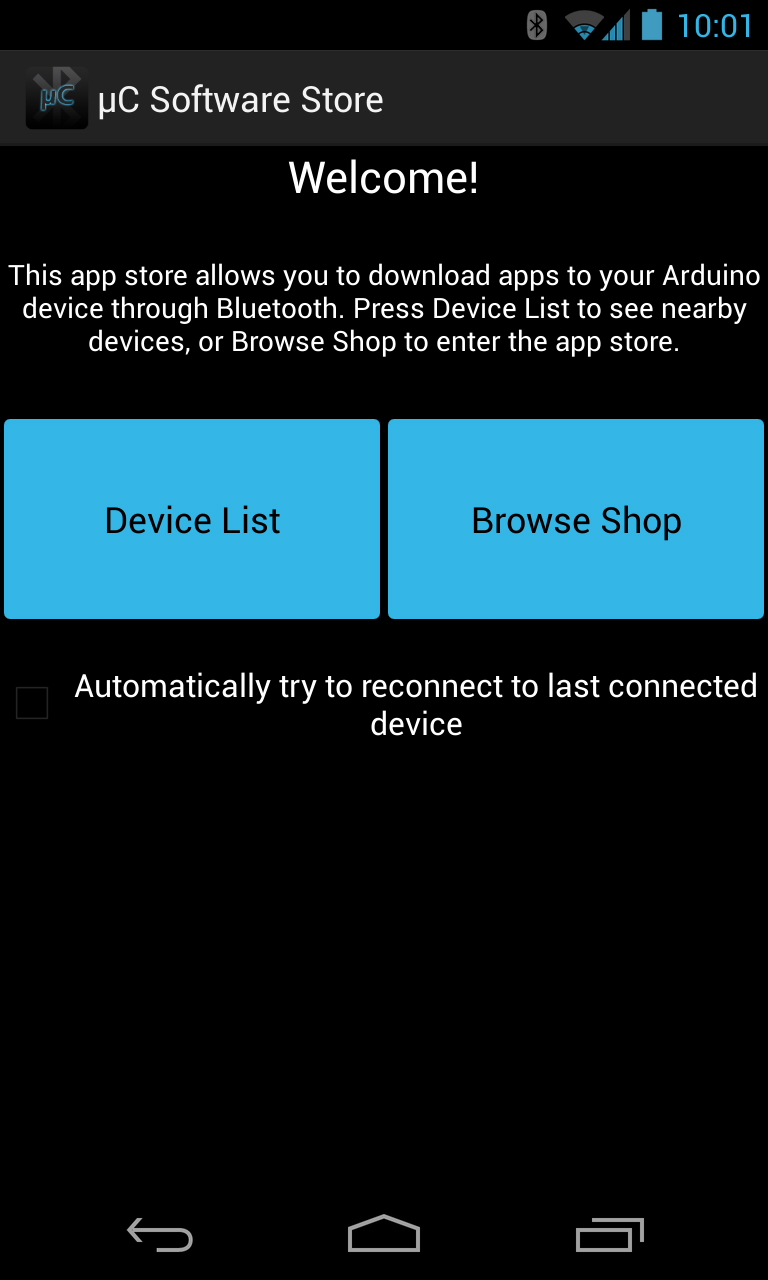
\includegraphics[width=0.5 \textwidth]{images/Screenshots/welcome_screen.png}
			\caption{The welcome screen of the $\mu$C Software Store.}
		\end{figure}

		After the first time the application was launched, the welcome screen will attempt to automatically reconnect to the last known connected device. This is an option which can be turned off in the settings. 
		\newpage
	\section{Device List}
		Upon selecting the ``Device List'' button from the welcome screen or from the action overflow, this screen will appear. On this screen, Bluetooth devices within the reach of the Android device will appear in a list. If the device you want to connect to doesn't show, or you do not want to connect to a device just yet, you can press either the ``Add device'' or ``Browse shop'' button respectively.\\
	\begin{figure}[H]
		\subfigure[]{
			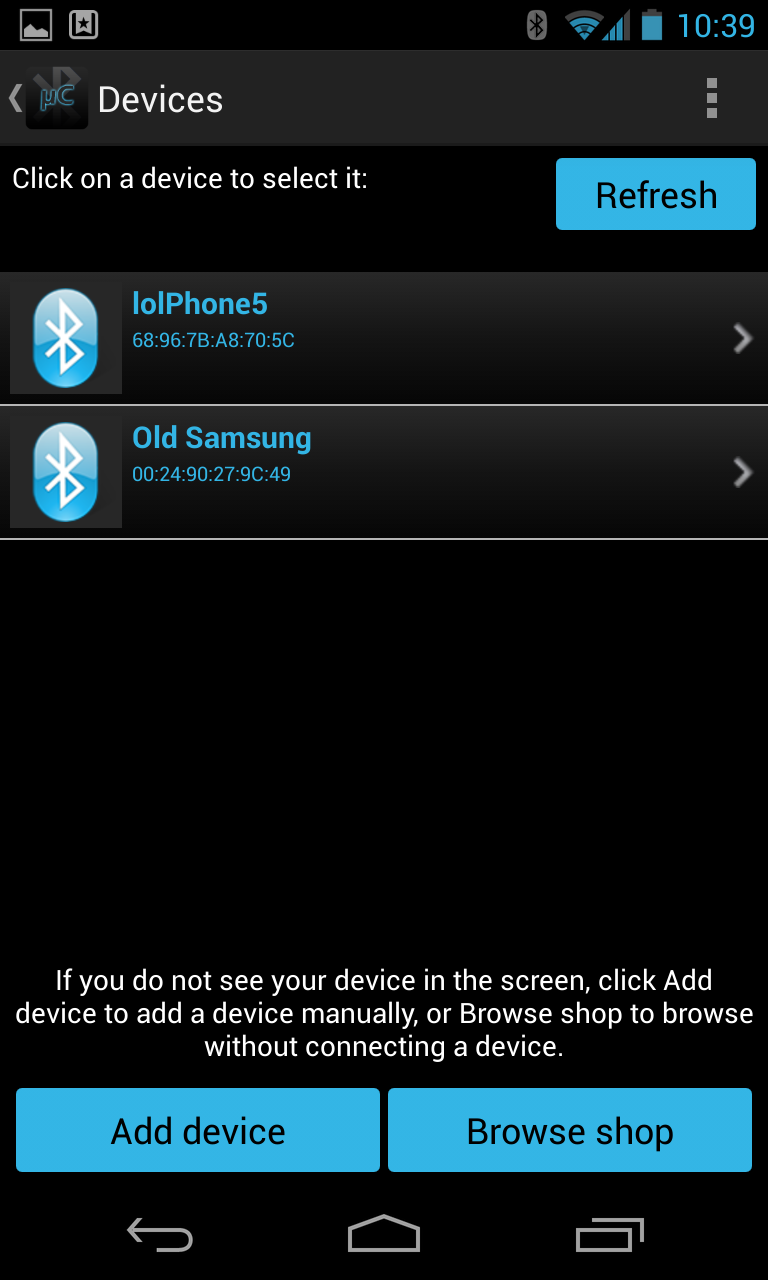
\includegraphics[width=0.5 \textwidth]{images/Screenshots/device_list.png}
			\label{fig:bt-list}
			}%
\hfill
		%nytt bilde med connected		
		\subfigure[]{
			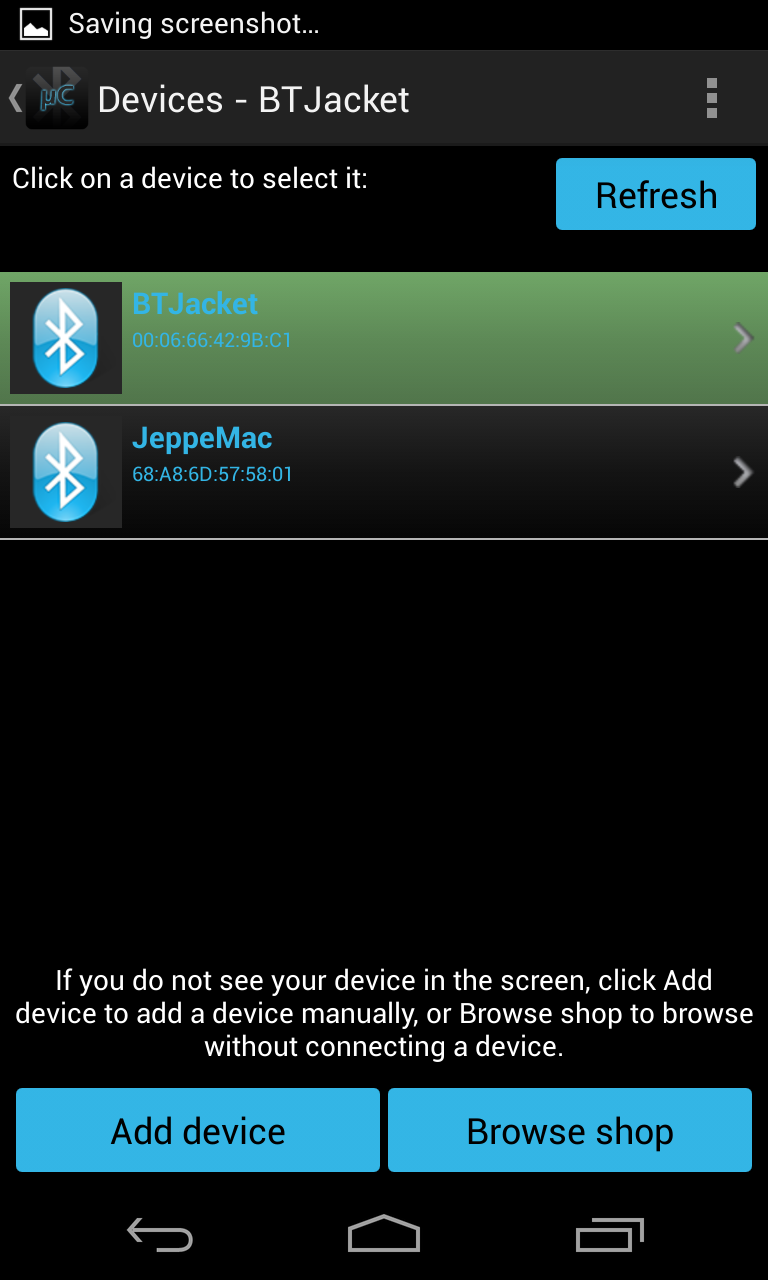
\includegraphics[width=0.5 \textwidth]{images/Screenshots/connected.png}
			\label{fig:bt-connected}
		}%
		\caption{\protect{\ref{fig:bt-list}} The device list with Bluetooth devices. \protect{\ref{fig:bt-connected}} The device list when connected to a device.}
	\end{figure}

		 To connect to a device, simply press the appropriate device in the list and a connection will be established. Some devices require a password in order for connection to be made. In this case will selecting this device trigger a password input prompt. A dialog box will show whether or not the connection was sucecssfully established. The background of the now connected device in the list will turn green to indicate that it is connected. \\

		\subsection{Adding Device}
			Pressing the ``Add device'' button will give you a choice of how you want to add or connect to a device. You can attempt to connect to a device using either a QR Code or input a serial adress.
		%bilde
		\newline
		\begin{figure}[H]
			\centering
			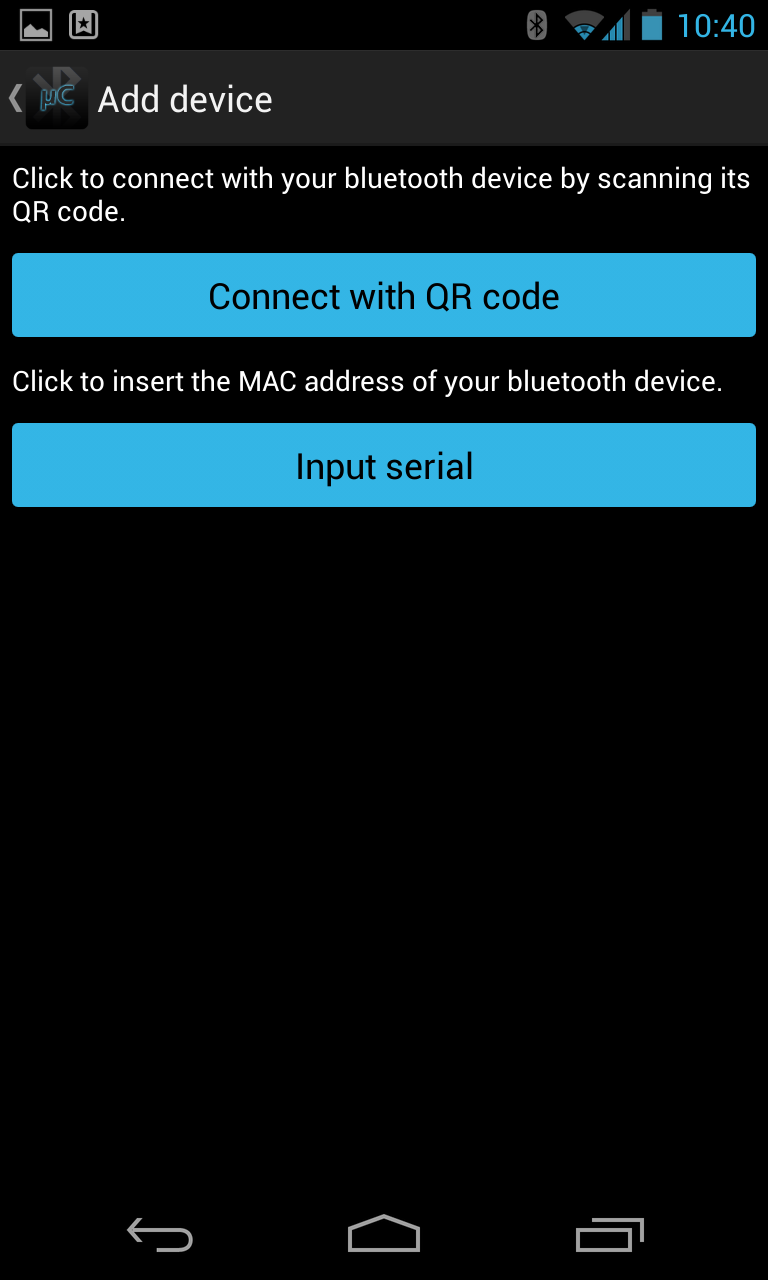
\includegraphics[width=0.5 \textwidth]{images/Screenshots/add_device.png}
			\caption{The options for adding devices}
		\end{figure}

			\subsubsection{QR Code}
				In order for you to connect with a QR Code, an app external app for scanning QR Codes must first be installed on the Android device. This will allow you to scan a QR Code which will automatically connect to an Arduino device if valid connection information is provided by the QR Code.\\

			\subsubsection{Serial}
				A connection can also be created by typing in a serial, which is the MAC address of the Arduino device. This serial is six groups of hexadecimal digits, meaning 0-9 and a-f, each group separated by a colon (:). You have to include the colon when typing this address, but it is not case sensitive which means you do not have to worry about capital letters.\\

	\section{The Shop}
		The first choice in the shop is the category screen.\\
	\begin{figure}[H]
		%bilde av category view
		\subfigure[]{
			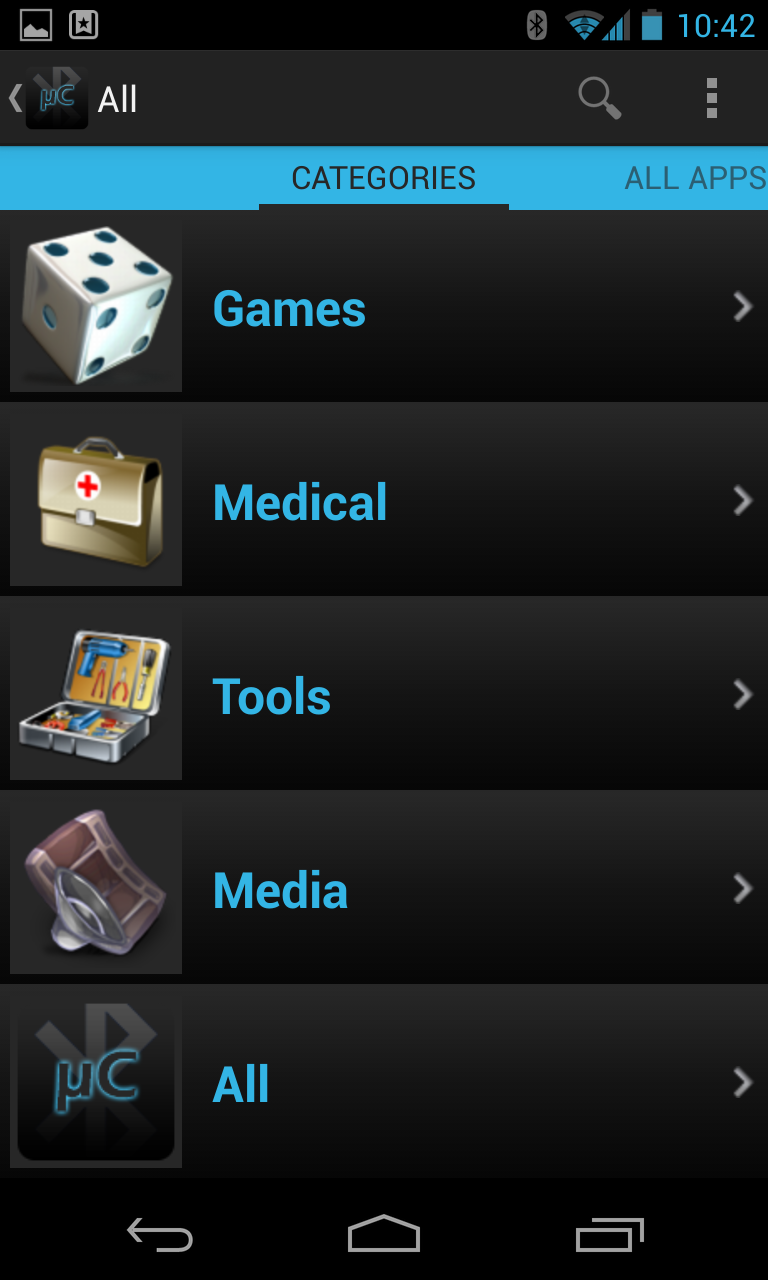
\includegraphics[width=0.5 \textwidth]{images/Screenshots/category_view.png}
			\label{fig:category-list}
		}%
		\hfill
		%bilde av all apps view	
		\subfigure[]{
			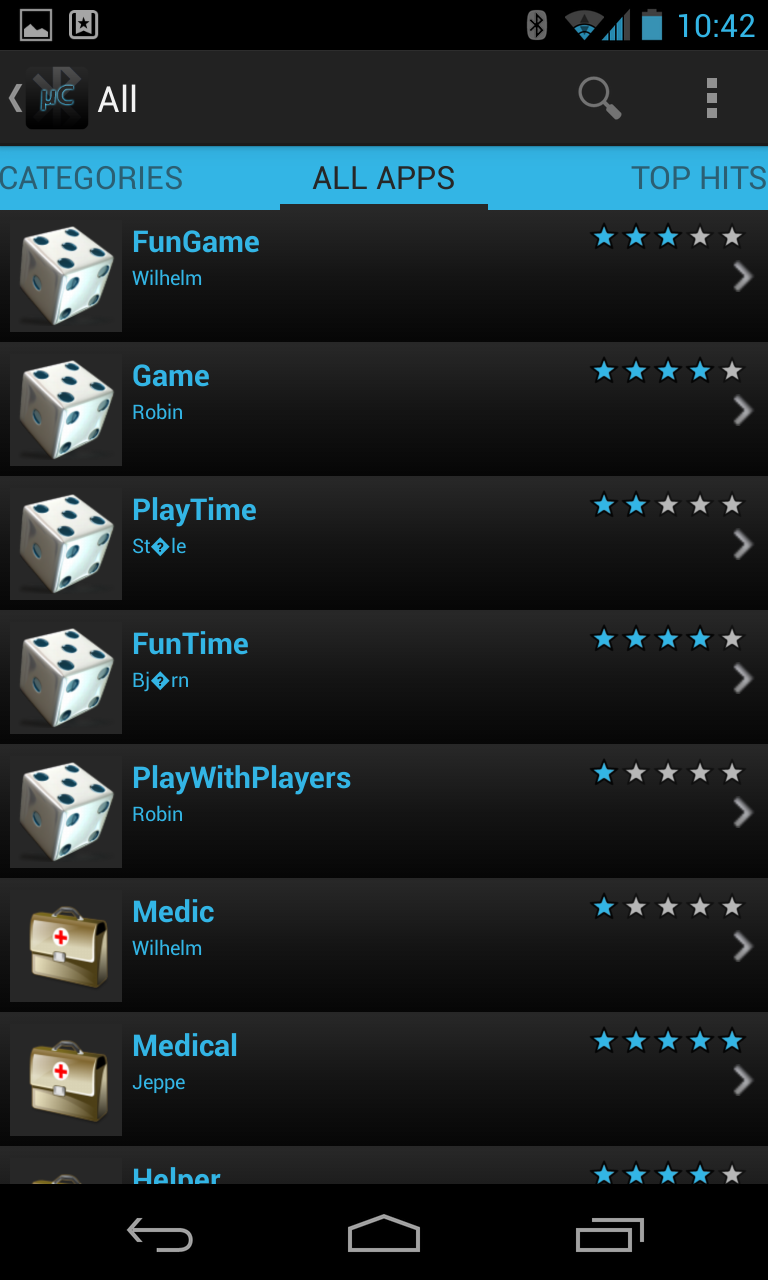
\includegraphics[width=0.5 \textwidth]{images/Screenshots/all_apps.png}
			\label{fig:all-apps}
		}%
		\caption{\protect{\ref{fig:category-list}} The device list with Bluetooth devices. \protect{\ref{fig:all-apps}} Screenshot from the shop with all apps shown.}
	\end{figure}
		
		You can filter through all of the apps in the store through these buttons. You can also browse all the apps together by pressing ``All''. There are two ways to sort the apps within the chosen category. Either not at all, which is the first screen that shows after selecting a category, or by the given rating. Each app within the category selected is now shown on the screen. The rating for each app, name of the app, name of the publisher, and the icon of the app is shown for all the apps. The user can go back to the categories by pressing the back button. \\

		\subsection{Searching}
			Wherever you are in the shop, you can start a search for an app you want. It doesn't matter how old or what buttons you have on your Android device, it is possible to start a search from all buttons and devices. The search results will show after pressing the search button, and if there are no results you will be back at the shop screen with a toast telling you there were no results.

	\section{App View}
	Upon selecting an app in the shop, you will be taken to the app view. This view displays more information about the app you selected, like required hardware, pictures, developer and most importantly, an install button. 
	%bilde
	\newline
	\begin{figure}[H]
		\centering
		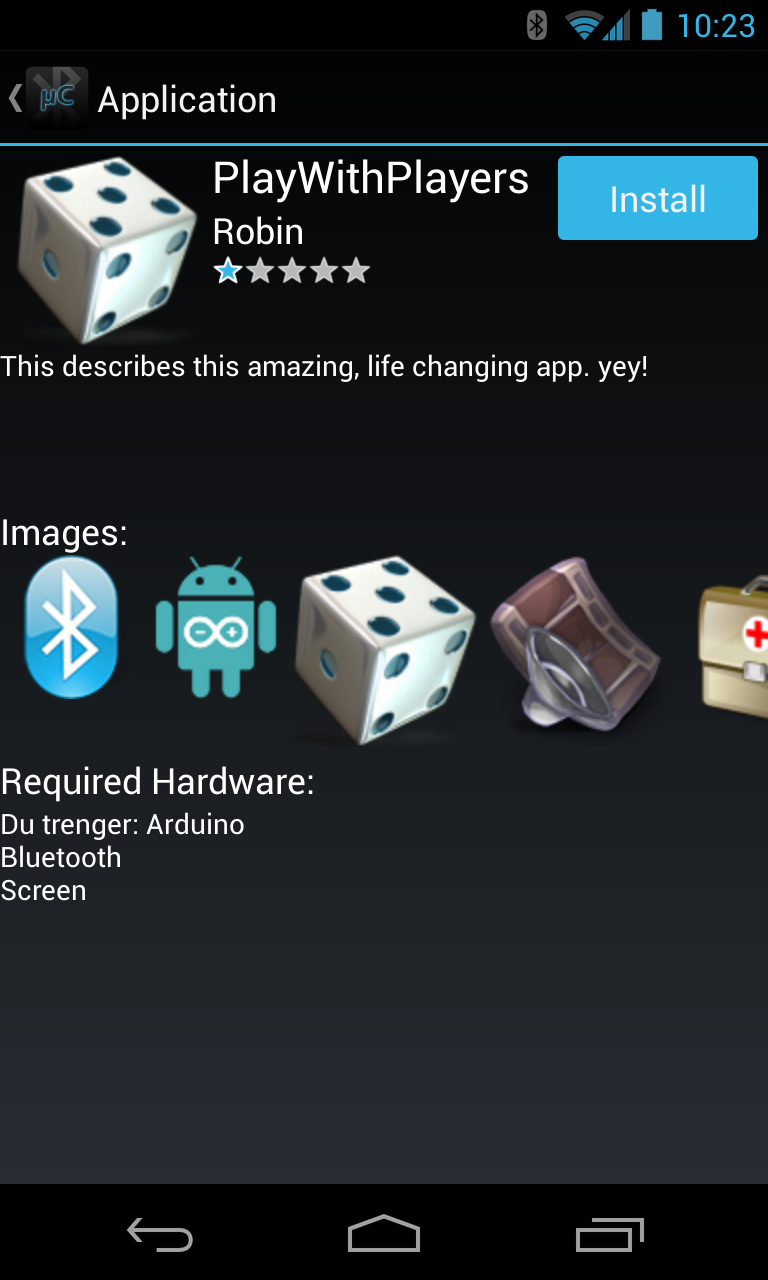
\includegraphics[width=0.5 \textwidth]{images/Screenshots/app_view.png}
		\caption{App View showing information about a single app}
	\end{figure}
	Upon pressing the ``Install'' button, as long as you are connected to an Arduino device, you will be first asked to confirm the action. If you do the install will begin. If, however, you are not connected to a device, a dialog will open with the options of either going back to the app view, or go directly do the device list to connect to a device.
\newpage
	\section{Settings}
	The settings available in $\mu$C Software Store are as follows:

	\begin{description}
		\item[Hide/Show incompatible] \hfill \\
			Allows you to hide/show all apps not compatible with the currently connected device.
		\item[Connected device] \hfill \\
			Shows the currently connected device. 
		\item[Automatically reconnect] \hfill \\
			 Controls whether the application should attempt to automatically reconnect at the welcome screen when reentering the application.
		\item[Hide other devices]\hfill \\
		Allows the option of hiding/showing devices in the device list which does not properly identifies themselves as an Arduino device. 
	\end{description}
